\chapter{Temperature and the Gas Laws}


\section{The Physics of Gases}
Why does a bike tire feel warm after you pump it up? Why does an aerosol can get cold when you spray it? How does an air conditioner pump heat out of a hot house? The answers all come from thinking about a gas as the motion of trillions of tiny molecules.

Imagine a balloon full of helium. Each helium atom zips around, bouncing off the others and off the rubber. Now, let us say you start to heat the helium inside the balloon. As the temperature goes up, the molecules inside will start to move faster.

Remember that the kinetic energy of an object with mass $m$ and velocity $v$ is given by

\begin{equation}
    k = \frac{1}{2} m v^2
    \label{eq:ke}
\end{equation}
So, you could say ``As the temperature of the gas increases, the kinetic energy of the molecules increases.''  But a physicist would say ``The temperature of the gas is how we measure its kinetic energy.''
\index{kinetic energy}
\subsubsection{A Statistical Look At Temperature}\index{molecular speed distribution}

If you say ``This jar of argon gas is 25 degrees Celsius,'' you have told me about the \emph{average} kinetic energy of the molecules in the jar. 
However, some molecules are moving very slowly. Others are moving really, really fast. 

We could plot the probability distribution of the speeds of the molecules. For argon at 25 degrees Celsius, it would look like this:
\begin{figure}[H]
    \centering
    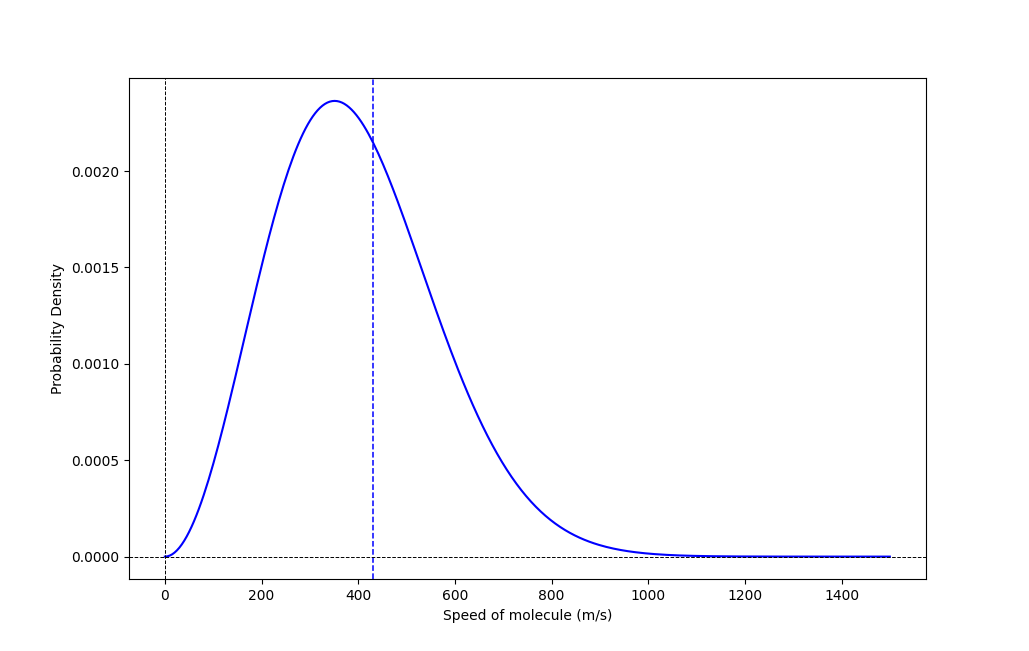
\includegraphics[width=\textwidth]{ar_plot.png}
    \caption{Probability distribution of molecular speeds for argon gas at 25 degrees Celsius.}
    \label{fig:argon_speed_distribution}
\end{figure}

The temperature, remember, is determined by the average kinetic energy of the molecules. Some molecules are moving slowly, and have less kinetic energy than the average. Some molecules are moving very quickly, and have more kinetic energy. The dotted line is the divider between the two groups: molecules moving at speeds to the left of the line have less kinetic energy than average; those on the right have more kinetic energy than average.

Where is that line? That is the RMS of the speeds of the molecules. That is, if we measured all the speeds of all the molecules $s_1, s_2, s_3, \ldots, s_n$, \index{root mean square speed}that line would be given by the root of the mean of the squares:

$$v_{rms} = \sqrt{\frac{1}{n} \left( s_1^2 + s_2^2 + s_3^2 + \ldots s_n^2 \right)}$$

If you have the same gas at a lower temperature, the distribution shifts toward zero: the peak becomes taller and narrower, and the tail of very fast molecules becomes much shorter.
In other words, fewer molecules have high speeds, and more molecules cluster near lower speeds. Let us look at an example.

Here is probability distribution of molecular speeds for argon gas at 25 degrees and -100 degrees Celsius.
\begin{figure}[H]
    \centering
    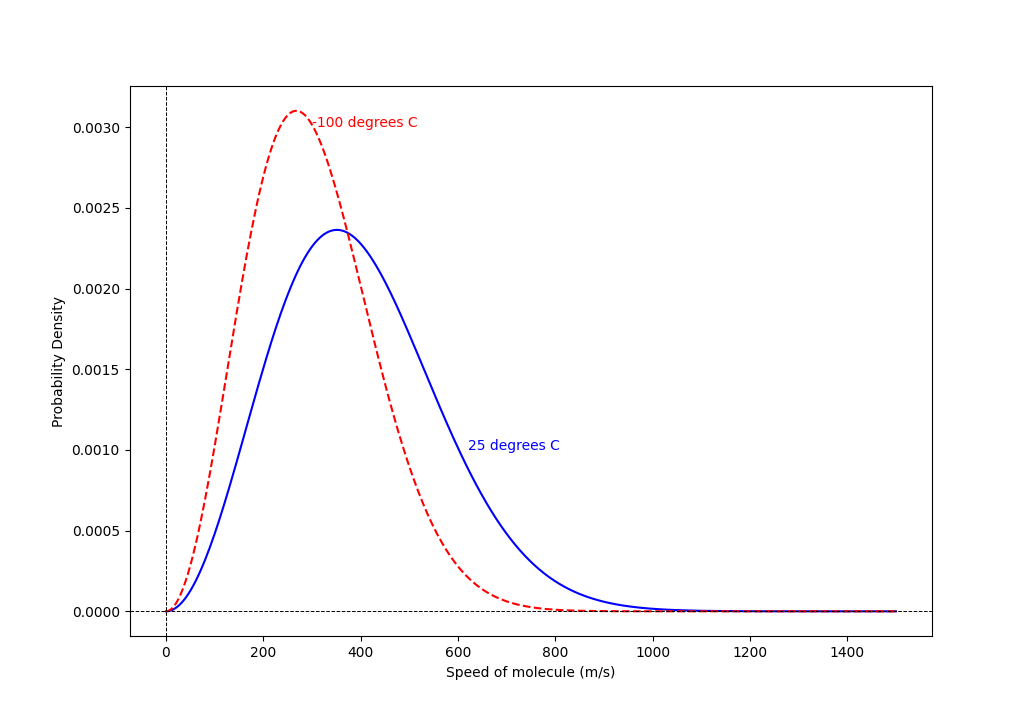
\includegraphics[width=\textwidth]{ar2_plot.png}
    \caption{Probability distribution of molecular speeds for argon gas at 25 degrees and -100 degrees Celsius.}
    \label{fig:argon_speed_distribution_2}
\end{figure}

\subsubsection{Absolute Zero and Degrees Kelvin}
\index{absolute zero}
If you keep lowering the temperature, eventually, all the molecules stop moving. This is known as \newterm{absolute zero} --- you
 cannot make anything colder than absolute zero. Absolute zero is $-273.15^\circ$ Celsius or $-459.67^\circ$ Fahrenheit.

In addition to Celsius and Fahrenheit, there is a third temperature system: Kelvin. Kelvin has the same scale as Celsius, but it starts at absolute zero (such that every value differs by 273.15).
So, 0 degrees Celsius is 273.15 kelvins, and 100 degrees Celsius is 373.15 kelvins.\index{Kelvin}

Any time you are working with the physics of temperature, you will use Kelvin.

Sometimes, when reading about gases, you will see \index{STP}``STP'' which stands for ``Standard Temperature and Pressure.'' STP is defined to be $0^\circ$ Celsius and 100 kPa.

\subsection{Temperature and Volume}

Let us say it is dawn, and a person is lying on a half-full air mattress in a field. The weight of the person will keep the pressure of the air inside constant (or pretty close). 
\begin{figure}[H]
    \centering
    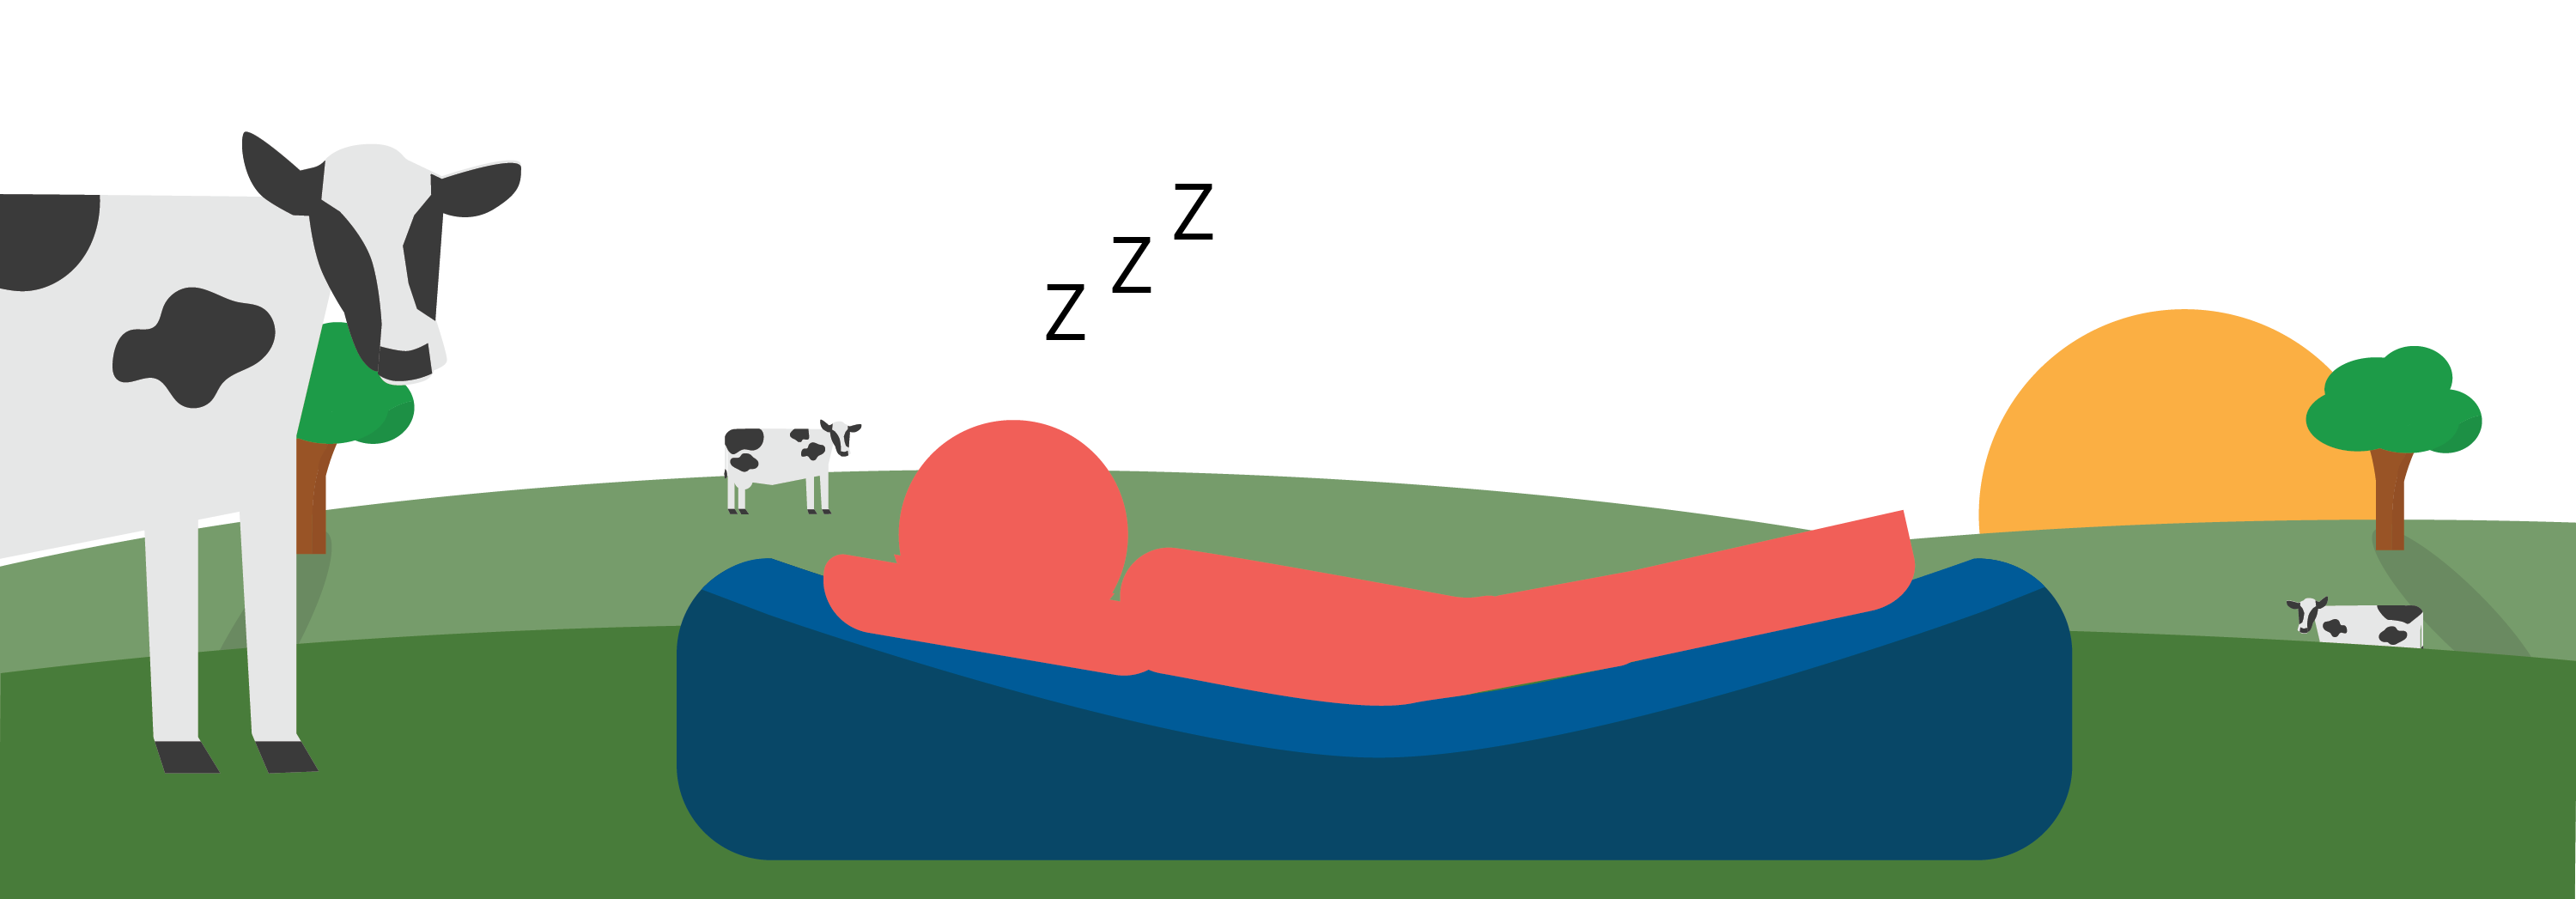
\includegraphics[width=\textwidth]{airMattress1.png}
    \caption{A person sleeping on an air mattress as the sun rises.}
    \label{fig:airMattress1}
\end{figure}


The molecules in the mattress are not entering or leaving that mattress. However, as the sun rises, the air inside will get warmer and expand. The person will be gently lifted by the expanding air. You might wonder: how much will the air expand?
% \begin{figure}[H]
%     \centering
%     
\includegraphics[width=\textwidth]{airMattress2.png}
%     \caption{The air mattress expands as the temperature increases.}
%     \label{fig:airMattress2}
% \end{figure}
\begin{figure}[H]
    \centering
    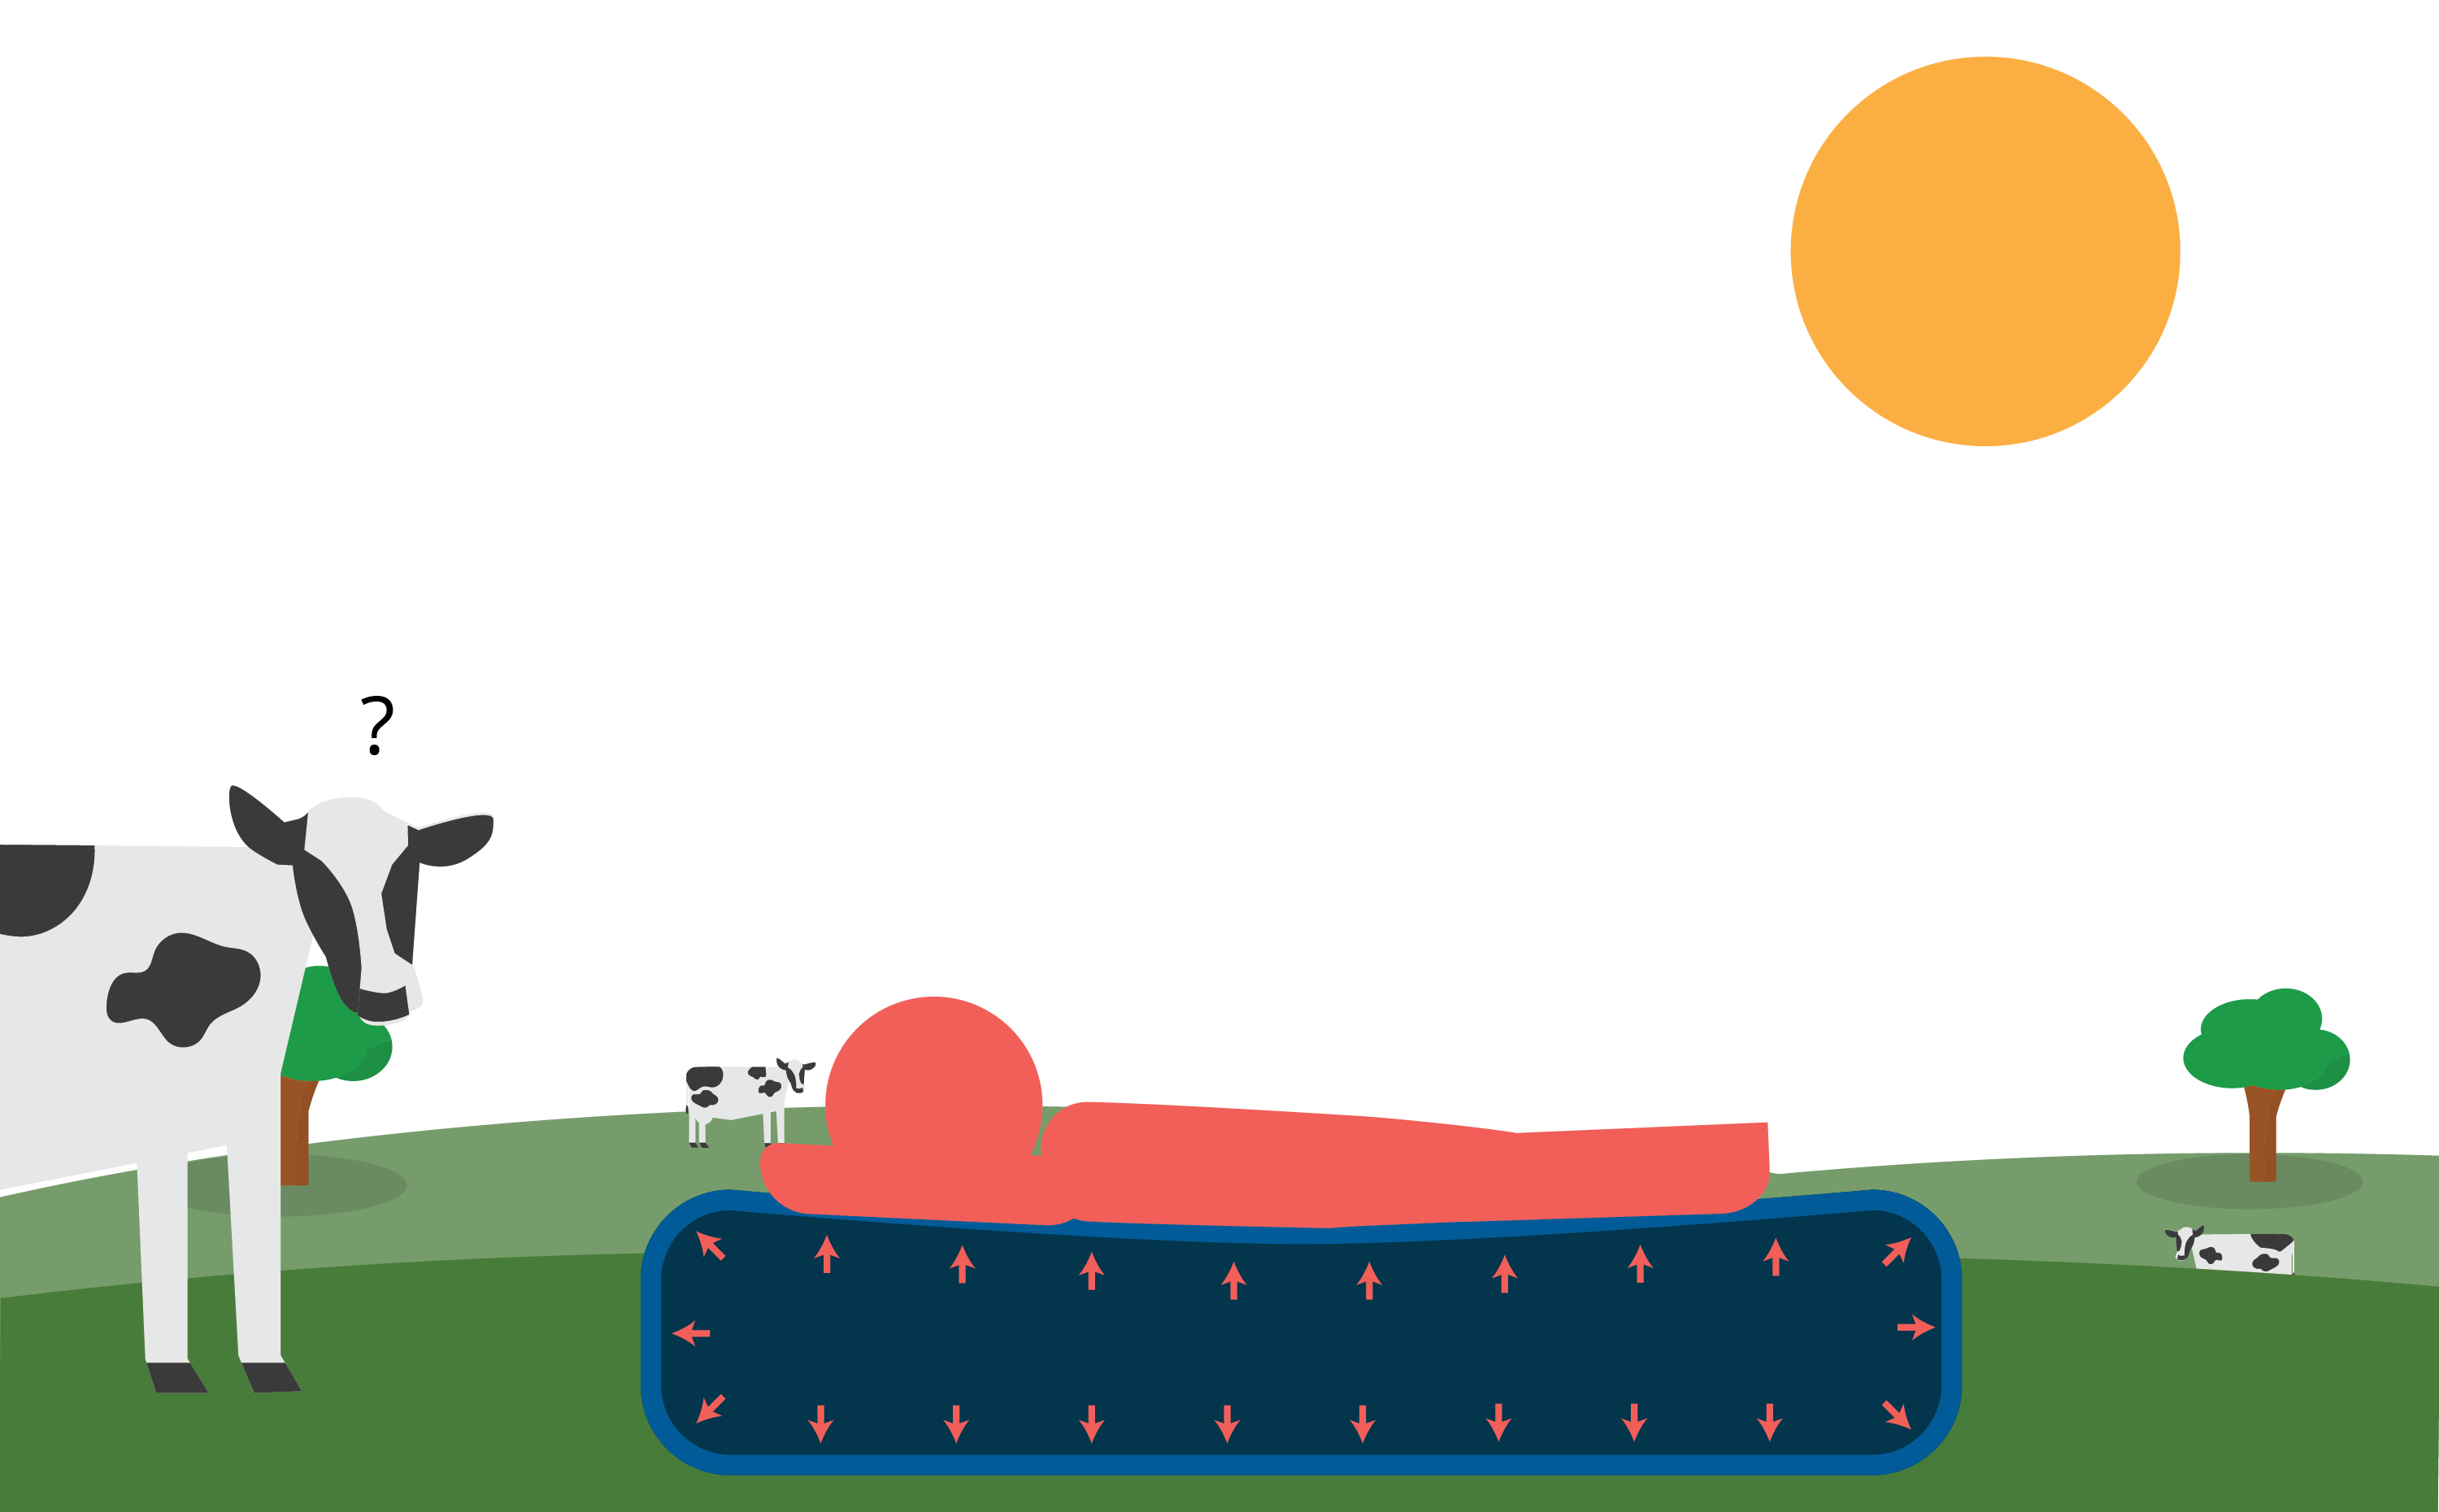
\includegraphics[width=\textwidth]{airMattress3.png}
    \caption{The air mattress inflates as the sun reaches its peak height in the sky.}
    \label{fig:airMattress3}
\end{figure}

If you have constant pressure and a constant number of molecules, the volume of the gas is proportional to the temperature in Kelvin:
\index{temperature and volume}\index{Charles's Law}
$$V \propto T$$

This is known as Charles's Law.

\begin{Exercise}[title={Temperature and Volume}, label=temp_vol]
 
At dawn, the air inside the mattress has a volume of 1000 liters and a temperature of 12 degrees Celsius.

At noon, that same air has a temperature of 28 degrees Celsius. The pressure on the gas has not changed at all.

What is the volume of the gas at noon?

\end{Exercise}
\begin{Answer}[ref=temp_vol]

First, we convert the temperatures into Kelvin: 
\begin{itemize}
\item Dawn: $12 + 273.15 = 285.15$
\item Noon: $28 + 273.15 = 301.15$
\end{itemize}

So, the temperature $T$ has increased by a factor of $\frac{301.15}{285.15} \approx 1.056$.

Thus, the volume of the air mattress has also increased by a factor of 1.056. 

This means that the air mattress that had a volume of 1000 liters at dawn will have a volume 1056 liters at noon.

\end{Answer}

Note: Volume and temperature are only proportional as long as the substance is a gas. We will talk about liquids and solids soon.

\subsection{Pressure and Volume}

As you increase the pressure on a gas, the molecules will get pushed closer together, and the volume will decrease.

% not necessarily an issue, but this exact example is talked about in chapter "atmos"
For example, if you put the cap on an empty plastic bottle and squeeze it.  As you put the gas inside the bottle under pressure, its volume will decrease. 

\begin{figure}[H]
    \centering
    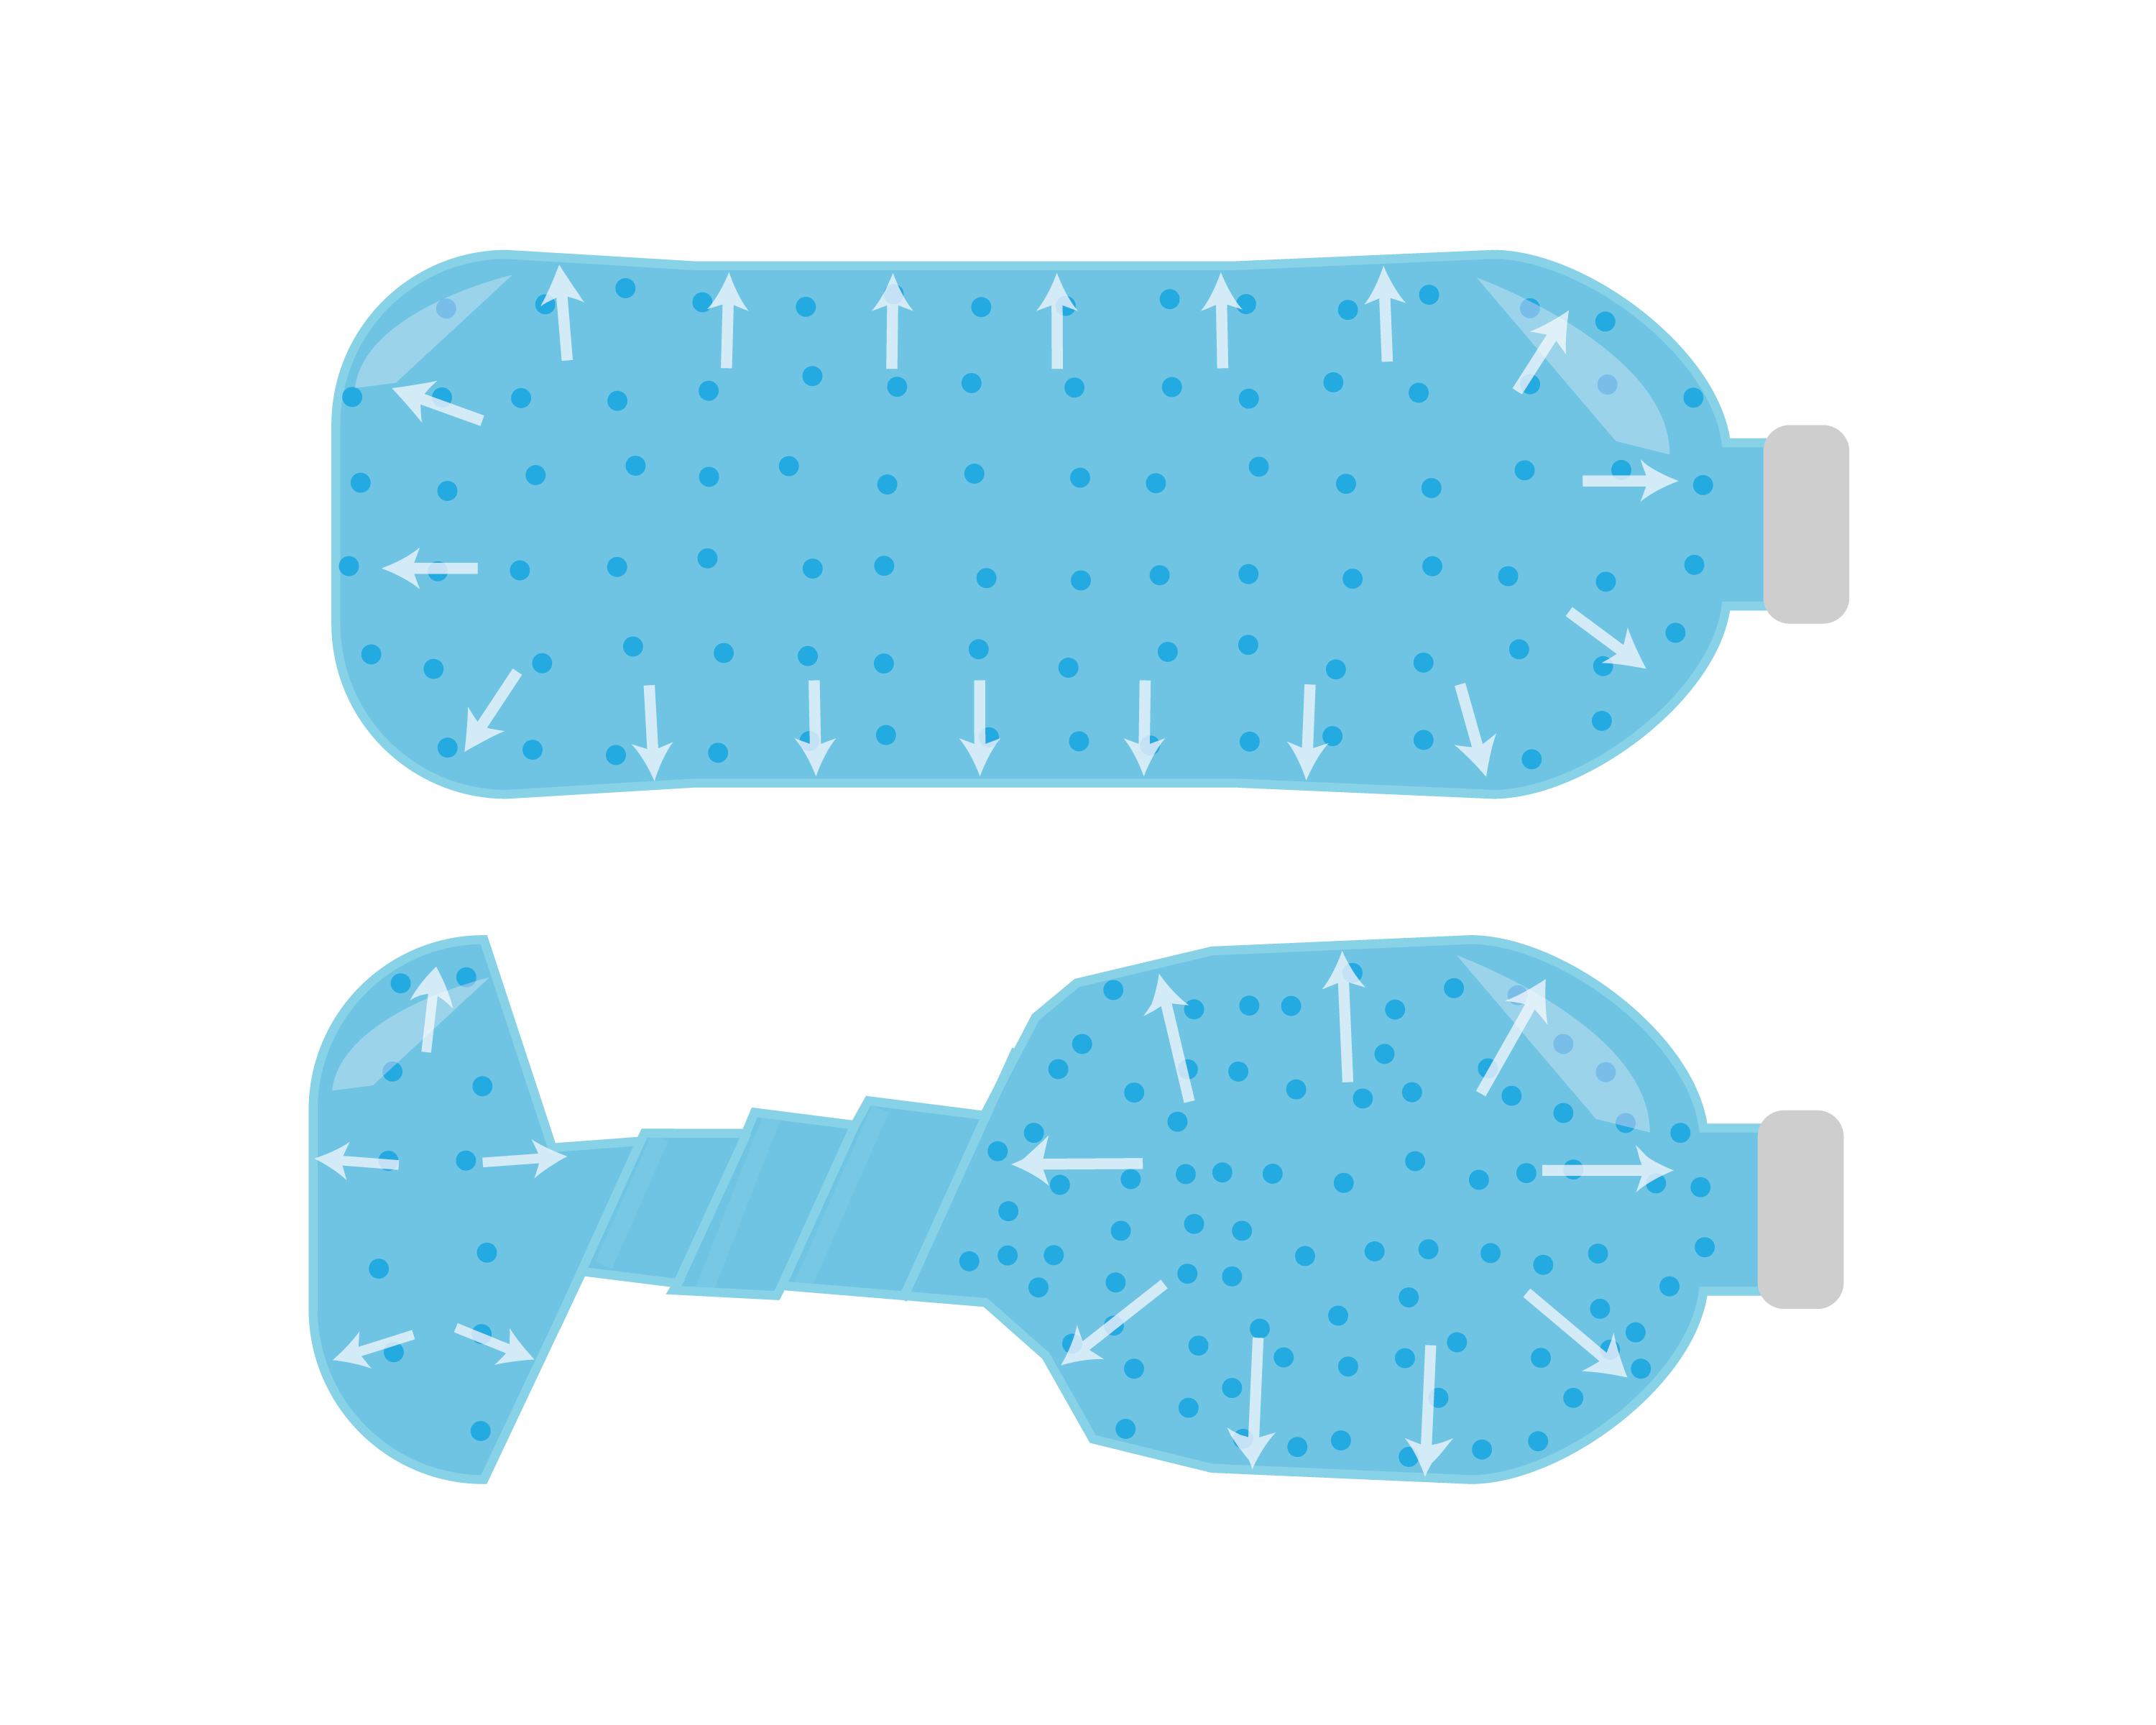
\includegraphics[width=0.75\textwidth]{waterBottle.png}
    \caption{The water bottle shrinks as it is put under pressure.}
    \label{fig:waterBottle}
\end{figure}


If you keep the number of molecules and the temperature constant, the pressure of the gas and its volume are inversely proportional:
\index{pressure and volume}\index{Boyle's Law}
$$P \propto \frac{1}{V}$$

This is known as Boyle's Law. ``But,'' you say with disbelief, ``if I increase the pressure on my empty water bottle from 5 kPa to 10 kPa, the volume inside will not decrease by half!''

Do not forget that the air inside the bottle is under 101 kPa of atmospheric pressure before you even start to squeeze it.

\begin{Exercise}[title={Pressure and Volume}, label=temp_vol_b]
 
At an altitude where the atmospheric pressure is 100 kPa, you seal air in a 1 liter water bottle.

Squeezing the water bottle, you raise the internal pressure by 20 kPa. What is the volume inside the bottle now?

\end{Exercise}
\begin{Answer}[ref=temp_vol_b]

What is the pressure in kPa? 
\begin{itemize}
\item Before squeezing: 100 kPa
\item While squeezing: 120 kPa
\end{itemize}

So, the pressure $P$ has increased by a factor of $\frac{120}{100} = 1.2$

$$1/1.2 \approx 0.833$$

The air in the bottle had a volume of 1 liter before squeezing, so it has a volume of 833 milliliters while being squeezed.

\end{Answer}

\subsection{The Ideal Gas Law}
\index{ideal gas law}
You are gradually getting an intuition for the relationship between the number of molecules, the volume, the pressure, and the temperature of a gas.
We can actually bring these together in one handy equation.

\begin{mdframed}[style=important, frametitle={Ideal Gas Law}]

$$PV = nRT$$

where:
\begin{itemize}
\item $P$ is the pressure in pascals
\item $V$ is the volume in cubic meters
\item $n$ is the number of molecules in moles
\item $R$ is the molar gas constant: 8.31446
\item $T$ is the temperature in Kelvin
\end{itemize}

(You can remember this as the "Pivnert.")

\end{mdframed}

From the name, you might predict the following: The Ideal Gas Law is not 100\% accurate. However, for most purposes, it works remarkably well. 

Notice that the ideal gas law says nothing about what kind of gas it is; it works regardless.

\begin{Exercise}[title={Ideal Gas Law}, label=ideal_gas]
 
You have a cylinder containing $O_2$. The chamber inside has a radius of 12 cm and a length of 50 cm. 
The temperature inside the cylinder is 20 degrees Celsius.
The pressure inside the tank is 600 kPa.

How many moles of $O_2$ are inside?

\end{Exercise}
\begin{Answer}[ref=ideal_gas]

First, let us convert the known values to the right unit:
\begin{itemize}
\item Radius = 0.12 m
\item Length = 0.5 m
\item $T = 20 + 273.15 = 293.15$ kelvins
\item $P = 600 \text{ kPa } = 600,000 \text{ Pa }$
\end{itemize}

The volume of the cylindrical chamber is $V = \pi r^2 h = \pi (0.12)^2 (0.5) \approx 0.0226$ m$^3$.

The Ideal Gas Law tells us that $PV = nRT$. We are solving for $n$.

$$n = \frac{PV}{RT} = \frac{(600,000)(0.0226)}{(8.31446)(293.15)} \approx 5.57 \text{ moles of } O_2$$

\end{Answer}

\subsection{Molecules Like To Stay Close to Each Other}\index{intermolecular forces}

When two molecules get close to each other a few things can happen:
\begin{itemize} 
\item They can under go a chemical reaction: electrons are exchanged or shared and a different molecule or molecules come into existence. 
This is the realm of chemistry, and we will not go into it in this course.
\item One or both of them have so much kinetic energy that they just pass each other or bounce off each other. This is what happens in a gas.
\item The two molecules can "stick" together. This is what happens in a liquid or a solid.
\end{itemize}

Why do they stick together if they are not combined in a chemical reaction?

First, they do not get \emph{too close}. If they get too close, their electron clouds repel each other with a strong force. 
This is what happens in a gas when two molecules bounce off of each other.

However, if the molecules are quite close to each other, there are forces that will attract them toward each other. 
These intermolecular forces are beyond the scope of this course, but they are called \index{van der Waals forces}Van der Waals forces and hydrogen bonds.  
The strength of these forces vary based on the two molecules involved. 

Which is why some of the matter around you is in gas form (molecules that do not stick together at the temperature and pressure you are living in because they have weak attractive forces) and some is non-gas 
(gangs of molecules with stronger attraction that makes them clump together as a liquid or a solid at that same temperature and pressure).

However, what if we change the temperature and pressure? We can change if and how the molecules clump together. 
This is known a \newterm{phase change}; We will cover it soon.


\section{Kinetic Energy and Temperature of a Gas}
As mentioned earlier in this chapter, for a particular gas, the temperature (in Kelvin) is proportional to the average kinetic energy of the individual molecules. 

Perhaps you want to warm 3 moles of helium gas (trapped in a metal cylinder) from 10 degrees Celsius to 30 degrees Celsius.  
How would you compute exactly how many Joules of energy this would require?

The amount of energy necessary to raise one mole of a molecule by one degree is known as \newterm{molar heat capacity}. \index{molar heat capacity}
(The molar heat capacity of liquid water, for example, is 75.38 J per mole-degree.)

With gases, there are actually two different possible situations:
\begin{enumerate}
\item Constant volume: As you heat the gas, the pressure and the temperature increase. This molar heat capacity is usually denoted as $C_{V,m}$. \index{heat capacity!constant volume}
\item Constant pressure: As you heat the gas, the temperature and the volume increase. This molar heat capacity is usually denoted as $C_{P, m}$.\index{heat capacity!constant pressure}
\end{enumerate}

All gases made up of one atom (Helium, for example, is a monoatomic gas) have the same values for $C_{V,m}$ and $C_{P,m}$:

$$C_{V,m} = \frac{3}{2}R \approx 12.47 \text{ Joules per mole-degree}$$

$$C_{P,m} = \frac{5}{2}R \approx 20.8 \text{ Joules per mole-degree}$$

(Remember that $R$ is the ideal gas constant $\approx 8.31446$ Joules per mole-degree.)

\begin{Exercise}[title={Warming Helium}, label=warming_helium]

You have 3 moles of helium. 
 
\begin{enumerate}

\item How many Joules would be required to warm 3 moles of helium gas by 20 degrees Celsius at constant volume? 

\item How many Joules would be required to warm 3 moles of helium gas by 20 degrees Celsius at constant pressure? 

\end{enumerate}


\end{Exercise}
\begin{Answer}[ref=warming_helium]

Constant volume: $E = C_{V,m} \, n \, \Delta T = (12.47)(3)(20) \approx 748$ joules.



Constant pressure: $E = C_{P,m} \, n \, \Delta T = (20.8)(3)(20) \approx 1247$ joules. (A change of 20 degrees Celsius is also a change of 20 kelvins.)
\end{Answer}

\subsection{Molecule Shape and Molar Heat Capacity}

We told you that gases made up of one atom have the same values for $C_{V,m}$ and $C_{P,m}$:

$C_{V,m} = \frac{3}{2}R \approx 12.47 \text{ Joules per mole-degree}$

$C_{P,m} = \frac{5}{2}R \approx 20.8 \text{ Joules per mole-degree}$

\index{Mayer's relation}For any molecule, it is generally true that 

$$C_{P,m} \approx C_{V,m} + R$$

It is also true that for any molecule, there is some integer $d$ such that

$$C_{V, m} \approx \frac{d}{2}R$$

For example, for all monoatomic gases, $d = 3$. For diatomic gases (like $N_2$ and $O_2$, $d$ is 5.

$d$ is known as the \index{degree of freedom}\newterm{degree of freedom} of the molecule. When you study chemistry, they will teach you to predict $d$ based on the shape of the molecule. 

Here are the relevant numbers for some gases you are likely to work with. (For molecules with three or more atoms, vibrations also store energy, so $C_{V,m}$ is only roughly a multiple of $\frac{R}{2}$.)

\begin{tabular}{r|c|c| c| c}
Gas & type & $C_{V,m}$ & $C_{P,m}$ & $d$\\
\hline
$He$ & monoatomic & 12.4717 & 20.7862 & 3 \\
$Ar$ & monoatomic & 12.4717 & 20.7862 & 3 \\
$O_2$ & diatomic & 21.0 & 29.38 & 5\\
$N_2$ & diatomic & 20.8 & 29.12 & 5\\
$H_2O$ (water vapor) & 3 atoms & 28.03 & 37.47 & 7 \\
$CO_2$ & 3 atoms & 28.46 & 36.94 & 7\\
\end{tabular}

\subsection{Kinetic Energy and Temperature}

For a sample of a gas, we can calculate its kinetic energy based on its molar heat capacity, the number of molecules, and the temperature:

$$E_K = C_{V,m} n T$$

where

\begin{itemize}
\item $E_K$ is the kinetic energy in Joules
\item $C_{V,m}$ is the molar heat capacity of the gas at constant volume
\item $n$ is the number of molecules in moles
\item $T$ is the temperature in Kelvin
\end{itemize}


\begin{Exercise}[title={Warming Helium Revisited}, label=warming_helium2]

How much kinetic energy does 3 moles of helium have at 10 degrees Celsius?

How much kinetic energy does 3 moles of helium have at 30 degrees Celsius?

What is the difference?

\end{Exercise}
\begin{Answer}[ref=warming_helium2]

10 degrees Celsius is 283.15 kelvins. 30 degrees Celsius is 303.15.

For any gas:

$$E_K =C_{V,m} n T$$

And $C_{V,m} = 12.47$ for all monoatomic gases.

So, the energy at 10 degrees Celsius:

$$E_1 = (12.47)(3)(283.15) = 10,594 \text{ Joules}$$

The energy at 30 degrees Celsius:

$$E_2 = (12. 47)(3)(303.15) = 11,342 \text{ Joules}$$

The difference?

$$E_2 - E_1 = 11,342 - 10,594  = 748 \text{ Joules }$$

Which is consistent with your earlier exercise.

\end{Answer}

\subsection{Why is $C_{V,m}$ different from $C_{P,m}$?}

What if, instead of keeping the volume constant while we heat the molecules in the helium tank, we keep the pressure constant and let the gas expand? 
The change in kinetic energy is the same: 748 Joules.

However, we know that the molar heat capacity if we keep pressure constant is $\frac{5}{2}R$, so heating will require $\frac{5}{2}R(3)(20) = 1247$ Joules. 

What happened to the 499 missing Joules!? Thermodynamics tells us energy is neither created nor destroyed, so it must have gone somewhere.

That energy was used pushing against the pressure as the gas expanded. For example, maybe the sample was in a balloon in space --- the extra energy stretched the surface of the balloon. 

The 499 joules went into the work of pushing the surroundings out of the way.  

\subsection{Work of Creating Volume Against Constant Pressure}

Let us imagine that you had a total vacuum (zero pressure) with a piston. As you pulled the piston out, you would be pulling against the atmospheric pressure. How much energy would that require?

If you increased the volume of the vacuum by $V$ against a pressure of $P$, you would do \index{work!pressure-volume}$VP$ work.

Let us check to make sure the 499 Joules mentioned above makes sense with this in mind.

No initial pressure was given in the problem, so let us just make one up and see how things work out: 100 kPa. Using the ideal gas law, the initial volume would be:

$$V_1 = \frac{n R T}{P} = \frac{(3)(8.31446)(283.15)}{100,000} = 0.07063\text{ cubic meters}$$

The volume after we heated the gas and let it expand against 100 kPa would be:

$$V_2 = \frac{n R T}{P} = \frac{(3)(8.31446)(303.15)}{100,000} = 0.07562\text{ cubic meters}$$

So, the volume increased by $0.07562 - 0.07063 = 0.00499$ cubic meters.  
Multiplying that by 100,000 pa, we get 499 Joules, as we expected!

\subsection{Why does a gas get hotter when you compress it?}

Now, imagine that there is gas inside the piston and you push on the piston to compress that air.  The work that you do is converted into kinetic energy, and that kinetic energy raises the temperature of the gas.

For example, if you had two moles of argon gas in the piston, and you pushed the piston 0.1 meters with an average force of 50 newtons, you will have done 5 Joules of work.

How much would 5 Joules raise the temperature of 2 mole of a monoatomic gas? 

$$\Delta T = \frac{5}{(2)(C_{V,m})} = 0.2\text{ K}$$ 

It works both ways: Compression makes a gas hotter; decompression makes a gas colder. You can sometimes experience the heat of compression when you pump up a bicycle tire --- as you pump the tire will get warmer.

If you compress or decompress a gas without letting any heat enter or depart, we say the compression or decompression was \index{adiabatic process}\newterm{adiabatic}. In order to solve any interesting problems about heating/cooling due to compression/decompression, you will need to assume the process was adiabatic.

When a spacecraft enters the atmosphere, it has to deal with a lot heat. Some people assume that heat is due to friction of the air rubbing against the 
spacecraft at over 7,000 meters per second. Actually, most of the heat is due to the compression of the air as it gets pushed out of the way of the spacecraft.

\subsection{How much hotter?}

Let us say you have an accordion-like container filled with helium at 100 kPa (about 1 atmosphere) and 300 kelvins. It holds 2 cubic meters. You then you put it in a vice and quickly compress it down to 0.5 cubic meters. Assuming it was adiabatic, how hot would the gas inside be after the compression?

Here is the challenging part: As you crush the container, the temperature and the pressure in the container are both increasing. So, as you go, it gets harder and harder to crush. Each milliliter of volume that you eliminate requires a little more work than the milliliter before.

Let us simulate the process in Python, after which we will give you the formula. 

In the simulation, you will start with an initial volume of 2 cubic meters and crush it down to 0.5 cubic meters in 40 steps. At each step you will recalculate the temperature and pressure.

Next, you will plot the results. Make a file called \filename{gas\_crunch.py}:

\begin{minted}{python}
import numpy as np
import matplotlib.pyplot as plt

V_initial = 2.0 # cubic meters
V_final = 0.5 # cubic meters
step_count = 40 # steps

T_initial = 300.0 # kelvin
P_initial = 100000 # pascals

# Constants
R = 8.314462618 # ideal gas constant
C_v = 3.0 * R / 2.0 # molar heat capacity (constant volume)

# Compute the number of moles
n = P_initial * V_initial/(R * T_initial) 
print(f"The container holds {n:.2f} moles of helium")

# How much volume do we need to eliminate in each step? 
# (in cubic meters)
step_size = (V_initial - V_final) / step_count

# For recording the state for each step
data_log = np.zeros((step_count, 3))

# Variables to update in the loop
V_current = V_initial
T_current = T_initial
P_current = P_initial

for i in range(step_count):
  # Record the current state
  data_log[i,:] = [T_current, V_current, P_current/1000.0]

  # Find how much energy to make the step at the current pressure
  E_step = step_size * P_current

  # Find how big the change in temperature will be from that energy
  delta_T = E_step / (n * C_v)

  # Update the current temperature, volume, and pressure
  T_current += delta_T
  V_current -= step_size
  P_current = n * R * T_current / V_current

print(f"Iterative:{T_current:0.3f} K, {V_current:0.3f} m3, {P_current/1000.0:0.3f} kPa")

fig, axs = plt.subplots(3,1,sharex=True, figsize=(8, 6))
axs[0].set_xlim((0,step_count))
axs[0].plot(data_log[:,0], 'k', lw=0.2)
axs[0].plot(data_log[:,0], 'r.')
axs[0].set_ylabel("Temperature (K)")

axs[1].plot(data_log[:,1],'k', lw=0.2)
axs[1].plot(data_log[:,1], 'r.')
axs[1].set_ylabel("Volume (cubic m)")

axs[2].plot(data_log[:,2], 'k', lw=0.2)
axs[2].plot(data_log[:,2], 'r.')
axs[2].set_ylabel("Pressure (kPa)")

axs[2].set_xlabel("Step")

fig.savefig('tvpplot.png')
\end{minted}

When you run this, you will see how many moles of gas there are and reasonable estimates of the temperature, volume, and pressure:

\begin{minted}{python}
> python3 gas_crunch.py      
The container holds 80.18 moles of helium
Iterative:733.499 K, 0.500 m3, 977.999 kPa
\end{minted}

And a good plot of the intermediate values:
\begin{figure}[H]
    \centering
    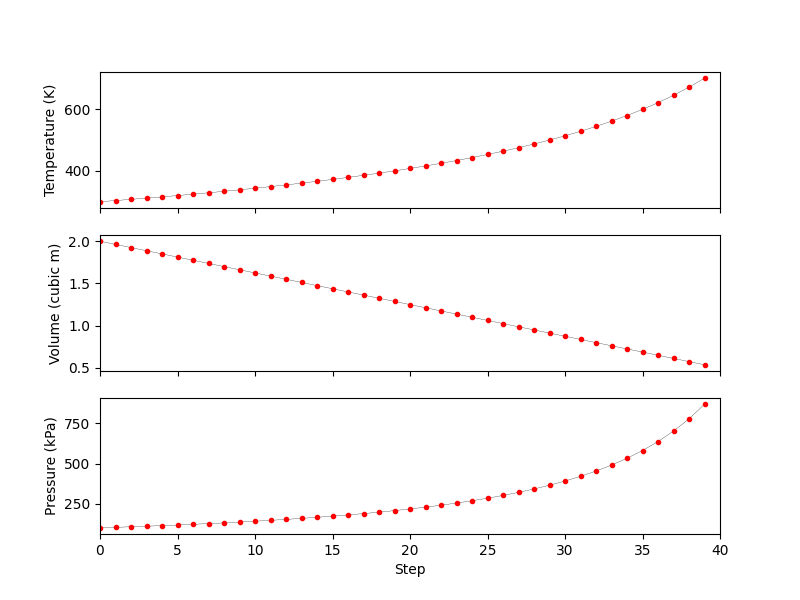
\includegraphics[width=\textwidth]{chunkplot1.png}
    \caption{Temperature, volume, and pressure during the compression, simulated in 40 steps.}
    \label{fig:chunkplot1}
\end{figure}

However, we will get better estimates if we break it up into 400 steps instead of 40. Change the line that defines the number of steps:

\begin{minted}{python}
step_count = 400 # steps
\end{minted}

Now the predicted temperature and pressure should be something like $753.603^\circ$ K and 1004.803 kPa.  (This is much closer to the correct result: 755.953 K and 1007.937 kPa.)

What if you break it into 400,000 steps? Now, the result should be really, really close to correct. And the plot is quite accurate:
\begin{figure}[H]
    \centering
    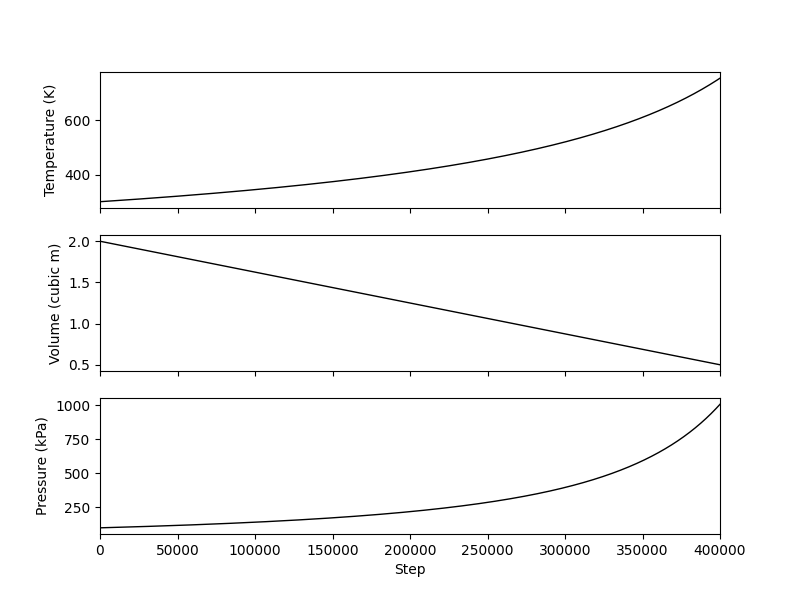
\includegraphics[width=\textwidth]{chunkplot2.png}
    \caption{The same compression simulated with many more steps.}
    \label{fig:chunkplot2}
\end{figure}

(You can comment out the lines that make the red dots on the graphs. No
one wants to see 400,000 red dots.)

It is inefficient to have to do long simulations to guess the final temperature and pressure. Fortunately, there are two handy rules you can use to skip this:
\index{adiabatic compression}
\index{adiabatic decompression}
\begin{mdframed}[style=important, frametitle={Adiabatic Compression and Decompression}]

Let 

$$\gamma = \frac{C_{P,m}}{C_{V,m}}$$

In an adiabatic compression or decompression, $P$ and $V$ change, but

$$P \left(V^\gamma \right)$$

stays constant.

Also 

$$T \left(V^{\left( \gamma - 1 \right)} \right)$$

stays constant

\end{mdframed}

For a monoatomic gas:

$$\gamma = \frac{C_{P,m}}{C_{V,m}} = \frac{5}{3}$$

$$\gamma - 1 = \frac{2}{3}$$

Before the compression: 

$$T \left(V^{\left( \gamma - 1 \right)} \right) = 300 \left( 2^{0.6667} \right) = 476.22$$

After the compression it has to be the same:

$$T \left(V^{\left( \gamma - 1 \right)} \right) = T \left( 0.5^{0.6667} \right) = 476.22$$

Thus 

$$T = 755.95\text{ K}$$

We can then use the ideal gas law to solve for the final pressure:

$$P = \frac{n R T}{V} = \frac{(80.18)(8.31446)(755.95)}{0.5} = 1007937 \text{ pascals}$$

That is hot! As you let it cool back down to 300 kelvins, how much heat would be released? 

$$E = C_{V,m} n \Delta T = (12.47)(80.2)(755.95 - 300) \approx 456 \text{ kJ}$$

\subsection{How an Air Conditioner Works}\index{air conditioner}

Once again, imagine the accordion-like container filled with helium. Let us say you walked it outside and compressed it from 2 cubic meters to 0.5 cubic meters in a vise. The container would get to 755.95 kelvins. You keep it compressed in the vise, but let it cool down outside. When it gets back to 300 kelvins, you walk it back inside.

Now, without letting any molecules in or out of the container, you release the vise. The gas is decompressed and gets very cold. How cold? Cold enough to accept about 456 kJ of kinetic energy from your house. That is, it would absorb heat from your house until the gas inside was the same temperature as your house.

So, you walk outside with your accordion and your vise, and repeat:
\begin{enumerate}
\item Compress the gas outside.
\item Let the hot gas cool down outside.
\item Walk the room-temperature compressed gas inside.
\item Decompress the gas inside.
\item Let the cold gas warm up inside.
\end{enumerate}

You could keep your house cool on a hot day this way. This is not unlike how an air conditioner works.

There is a hose filled with refrigerant that does a loop: 
\begin{itemize}
\item Outside, the refrigerant is compressed and allowed to cool to the outside temperature. (Usually there is a big fan blowing on a coil of refrigerant to speed the process.)
Inside, the refrigerant is decompressed and allowed to warm to the inside temperature. (Usually there is a big fan blowing the air of the home past a coil of refrigerant to speed the process.)
\end{itemize}

In each pass of the loop, the refrigerant absorbs some of the kinetic energy from inside the house, and releases it on the outside.

This same mechanism can be used to heat your house. (Units that both heat and cool are known as \index{heat pump}\newterm{heat pumps}.) 
The heat pump does the process backwards: The hot compressed refrigerant cools down inside. The cold decompressed refrigerant warms up outside.

The next chapter follows heat as it flows between objects and as it melts and boils matter.
